%% PNAStwoS.tex
%% Sample file to use for PNAS articles prepared in LaTeX
%% For two column PNAS articles
%% Version1: Apr 15, 2008
%% Version2: Oct 04, 2013

%% BASIC CLASS FILE
\documentclass{pnastwo}

%% ADDITIONAL OPTIONAL STYLE FILES Font specification
%\usepackage{pnastwoF}


%% OPTIONAL MACRO DEFINITIONS
\def\s{\sigma}
%%%%%%%%%%%%
%% For PNAS Only:
\url{www.pnas.org/cgi/doi/10.1073/pnas.0709640104}
\copyrightyear{2008}
\issuedate{Issue Date}
\volume{Volume}
\issuenumber{Issue Number}
%\setcounter{page}{2687} %Set page number here if desired
%%%%%%%%%%%%

\begin{document}

\title{Almost sharp fronts for the surface geostrophic equation}

\author{Roberta Graff\affil{1}{University of Cambridge, Cambridge,
United Kingdom},
Javier de Ruiz Garcia\affil{2}{Universidad de Murcia, Bioquimica y Biologia
Molecular, Murcia, Spain},
\and
Franklin Sonnery\affil{2}{}}

\contributor{Submitted to Proceedings of the National Academy of Sciences
of the United States of America}

%%%Newly updated.
%%% If significance statement need, then can use the below command otherwise just delete it.
\significancetext{RJSM and ACAC developed the concept of the study. RJSM conducted the analysis, data interpretation and drafted the manuscript. AGB contributed to the development of the statistical methods, data interpretation and drafting of the manuscript.}

\maketitle

\begin{article}
\begin{abstract}
{We use heat kernels or eigenfunctions of the Laplacian to construct
local coordinates on large classes of Euclidean domains and Riemannian
manifolds (not necessarily smooth, e.g. with $\mathcal{C}^\alpha$
metric). These coordinates are bi-Lipschitz on large neighborhoods of
the domain or manifold, with  constants controlling the distortion and
the size of the neighborhoods that depend only on natural geometric
properties of the domain or manifold. The proof of these results relies
on novel estimates, from above and below, for the heat kernel and its
gradient, as well as for the eigenfunctions of the Laplacian and their
gradient, that hold in the non-smooth category, and are stable with
respect to perturbations within this category. Finally, these coordinate
systems are intrinsic and efficiently computable, and are of value in
applications.}
\end{abstract}

\keywords{monolayer | structure | x-ray reflectivity | molecular electronics}

\abbreviations{SAM, self-assembled monolayer; OTS, octadecyltrichlorosilane}

\dropcap{I}n this article we study the evolution of ``almost-sharp'' fronts
for the surface quasi-geostrophic equation. This 2-D active scalar
equation reads for the surface quasi-geostrophic equation.
\begin{equation}
\mfrac{D \theta}{Dt}=\mfrac{\pr \theta}{\pr t} + u\cdot \nabla
\theta=0 \label{qg1}
\end{equation}
where,
\begin{equation}
 u=(u_1,u_2)=(-\mfrac{\pr \psi}{\pr y},\mfrac{\pr \psi}{\pr
x})\label{qg2} \end{equation}
and,
\begin{equation} (-\triangle)^{\f12}\psi=\theta \, ,\label{qg3} \end{equation}
For simplicity we are considering fronts on the cylinder, i.e. we
take $(x,y)$ in $\mathbb{R}/_{\displaystyle{\mathbb{Z}}}\times
\mathbb{R}$. In this setting we define $-\triangle^{-\f12}$ that
comes from inverting the third equation by convolution with the
kernel. To avoid irrelevant considerations at $\infty$ we
will take $\eta$ to be compactly supported
\[
\mfrac{\chi(u,v)}{(u^2+v^2)^{\f12}}+\eta(u,v)
\]
where $\chi (x,y)\ \epsilon\ C^{\infty}_{0},\,\,
\chi(x,y)=1 \hspace{8pt} \mbox{in} \hspace{5pt} |x-y|\leq r \,\,
\mbox{and}\,\, supp \chi$ is contained in $  \{|x-y|\leq R\} $
with $0<r<R<\frac{1}{2}$. Also $ \eta\ \epsilon\ C^{\infty}_0$,
$\eta(0,0)=0 $.

The main mathematical interest in the quasi-geostrophic equation
lies in its strong similarities with the 3-Euler equations. These
results were first proved by Constantin, Majda and Tabak, see
\cite{1}, \cite{2} and \cite{3} for more details. There
are several other research lines for this equation, both
theoretical and numerical. See  \cite{4}, \cite{5}, and
\cite{6}.
The question
about the regularity of the solutions for QG  remains as an open
problem.

Recently one of the authors has obtained the equation for the
evolution of sharp fronts (in the periodic setting), proving its
local well-posedness for that equation. (see \cite{ZhaZha} and
\cite{TSL} for more details). This is a problem in contour
dynamics. Contour dynamics for other fluid equations has been
studied extensively.


\section{Analysis of almost sharp fronts}
We begin our analysis on almost sharp fronts for the
quasi-geostrophic equation recalling the notion of weak solution.

For these solutions we have the following

\begin{definition}
A bounded function $\theta$ is a weak solution of QG if for any
$\phi\,\epsilon\,
C_0^{\infty}(\fdb\times\mathbb{R}\times[0,\vep])$ we have
\begin{eqnarray}
&&  \int_{\mathbb{R}^+\times\fd\times\mathbb{R}} \hspace{-25pt}
 \theta(x,y,t)\, \pr_t \phi
\,(x,y,t) dy dx dt+\nonumber\\
  & +&\int_{\mathbb{R}^+\times\fd\times\mathbb{R}}
\hspace{-26pt} \theta\,(x,y,t) u(x,y,t)\cdot\nabla\phi\,(x,y,t)
dydxdt = 0 \label{weaksol} \end{eqnarray}
where $u$ is determined by equations \eqref{qg2} and \eqref{qg3}.
\end{definition}

\subsection{Data Sources}
We are interested in studying the evolution of almost sharp fronts
for the QG equation. These are weak solutions of the equation with
large gradient ($\sim \displaystyle{ \inlinefrac{1}{\delta}}$, where $2
\delta$ is the thickness of the transition layer for $\theta$).

\section{Discussion}
\subsection{Cylindrical Case}
We are going to consider the cylindrical case here. We consider a
transition layer of thickness smaller than $2\delta$ in which
 $\theta$ changes from 0 to 1. (see Figure \ref{afoto}).That means we are considering $\theta$  of the form
\[
\theta  = 1   \mbox{ if }\quad  y\geq \varphi(x,t)+\delta
\]
\[
\theta \mbox{ bounded} \mbox{ if }\quad |\varphi(x,t)-y|\leq\delta
\]
\be \theta = 0  \mbox{ if }\quad  y\leq \varphi(x,t)-\delta
\label{theta} \ee
where $\varphi$ is a smooth periodic function and
$0<\delta<\frac{1}{2}$.

%For these solutions we have the following

\begin{theorem}
If the active scalar $\theta$ is as in \eqref{theta} and satisfies
the equation \eqref{weaksol}, then $\varphi$ satisfies the
equation
\begin{eqnarray}
\mfrac{\pr \varphi}{\pr t}(x,t)&=&\hspace{-2pt}\dst
\int_{\fd}\mfrac{\mfrac{\pr \varphi}{\pr x}(x,t)-\mfrac{\pr
\varphi}{\pr
u}(u,t)}{[(x-u)^{2}+(\varphi(x,t)-\varphi(u,t))^{2}]^{\f12}}\nonumber\\
&&
\chi(x-u,\varphi(x,t)-\varphi(u,t)) du \hspace{3pt} +
\nonumber\\
&+&\dst \int_{\fd} \Big{[}\mfrac{\pr \varphi} {\pr
x}(x,t)-\mfrac{\pr \varphi}{\pr u} (u,t)\Big{]}
\nonumber\\&&
\eta(x-u,\varphi(x,t)-\varphi(u,t)) du + Error
\end{eqnarray}
with $|Error|\leq C\, \delta | log\delta| $ where $C$ depends only
on $\|\theta\|_{L^{\infty}}$ and $\|
\nabla\varphi\|_{L^{\infty}}$.
\end{theorem}

\begin{remark}
Note that equation \eqref{theta} specifies  the function $\varphi$
up to an error of order $\delta$. Theorem 1 provides an evolution
equation for the function $\varphi$ up to an error of order
$\delta |log \delta|$.
\end{remark}

In order to analyze the evolution of the ``almost-sharp'' front we
substitute the above expression for $\theta$ in the definition of
a weak solution (see \eqref{weaksol}). We use the notation $X =O(
Y)$ to indicate that $|X|\leq C |Y|$ where the constant $C$
depends only on $\|\theta\|_{L^{\infty}}$, $\|
\nabla\varphi\|_{L^{\infty}}$ and $\|\phi\|_{C^1}$, where $\phi$
is a test function appearing in Definition 1.

We consider the 3 different regions defined by the form on
$\theta$. Since $\theta=0$ in the region I the contribution from
that region is 0, i.e.
\[
  \int_{I\times \mathbb{R}}
 \theta(x,y,t)\, \pr_t \phi
\,(x,y,t) dy dx dt+  \]
\[
   +\int_{I\times \mathbb{R}}
 \theta\,(x,y,t) u(x,y,t)\cdot\nabla\phi\,(x,y,t) dydxdt = 0
\]

As for the region II
\[
\int_{II\times \mathbb{R}} \theta (x,y,t) \pr_t\phi (x,y,t)dx dy
dt = O(\delta)
\]
since $\theta$ is bounded and hence $O(1)$, and the area of the
region II is $O(\delta)$. As for the second term
\[
\int_{II\times \mathbb{R}} u \theta \nabla \phi dx dy dt =
O(\delta log(\delta))
\]

To see this, we fix $t$. We must estimate
\[
\int_{\mathbb{R}^2} u\cdot(\mathbb{1}_{II}\theta\nabla\phi) dx dy
\]
We are left to estimate the terms
\[
\int_{III\times \mathbb{R}} \theta \pr_t\phi dx dy
dt+\int_{III\times \mathbb{R}} \theta u_f\cdot \nabla \phi dx dy
dt=:A+B
\]

\subsection{Observations}
The following observations can be made form the numerical experiments
described in this section, and are consistent with the results
of more extensive experimentation performed by the authors:
\begin{itemize}
\item The CPU times in Tables 1--3 are compatible with the estimates in
formulae {\bf 14}, {\bf 16}, and {\bf 23}.
\item
The precision produced by each of Algorithms {\bf I} and {\bf II}
is similar to that provided by formula {\bf 3}, even when
$\omega_{k+1}$ is close to the machine precision.
\end{itemize}




\begin{materials}
\section{Digital RNA SNP Analysis} A real-time PCR assay was designed
to amplify {\it PLAC4} mRNA, with the two SNP alleles being discriminated
by TaqMan probes. {\it PLAC4} mRNA concentrations were quantified in
extracted RNA samples followed by dilutions to approximately one target
template molecule of either type (i.e., either allele) per well.
Details are given in the {\it SI Materials and Methods}.

\section{Digital RCD Analysis} Extracted DNA was quantified by
spectrophotometry (NanoDrop Technologies, Wilmington, DE) and diluted to a
concentration of
approximately one target template from either chr21 or ch1 per well.
\end{materials}

\appendix[Estimating the Spectral Norm of a Matrix]
In this appendix we describe a method for the estimation of the spectral norm
of matrix $A$. The method does not require access to the individual
entries of $A$; it requires only applications of $A$ and $A$* to vectors.
It is a version of the classical power method. Its probabilistic
analysis summarized below was introduced fairly recently in refs. 13
and 14. This appendix is included here for completeness.


\appendix
This is an example of an appendix without a title.

\begin{acknowledgments}
This work was partially supported by
Spanish Ministry of Science and Technology Grant BFM2002-02042 (to D.C. and
J.L.R.) and by National Science Foundation Grand DMS-0245242 (to C.F.).
\end{acknowledgments}

\begin{thebibliography}{10}
\bibitem{BN}
M.~Belkin and P.~Niyogi, {\em Using manifold structure for partially
  labelled classification}, Advances in NIPS, 15 (2003).

\bibitem{BBG:EmbeddingRiemannianManifoldHeatKernel}
P.~B\'erard, G.~Besson, and S.~Gallot, {\em Embedding {R}iemannian
  manifolds by their heat kernel}, Geom. and Fun. Anal., 4 (1994),
  pp.~374--398.

\bibitem{CLAcha1}
R.R.~Coifman and S.~Lafon, {\em Diffusion maps}, Appl. Comp. Harm. Anal.,
  21 (2006), pp.~5--30.

\bibitem{DiffusionPNAS}
R.R.~Coifman, S.~Lafon, A.~Lee, M.~Maggioni, B.~Nadler, F.~Warner, and
  S.~Zucker, {\em Geometric diffusions as a tool for harmonic analysis and
  structure definition of data. {P}art {I}: Diffusion maps}, Proc. of Nat.
  Acad. Sci.,  (2005), pp.~7426--7431.

\bibitem{Clementi:LowDimensionaFreeEnergyLandscapesProteinFolding}
P.~Das, M.~Moll, H.~Stamati, L.~Kavraki, and C.~Clementi, {\em
  Low-dimensional, free-energy landscapes of protein-folding reactions by
  nonlinear dimensionality reduction}, P.N.A.S., 103 (2006), pp.~9885--9890.

\bibitem{DoGri}
D.~Donoho and C.~Grimes, {\em Hessian eigenmaps: new locally linear
  embedding techniques for high-dimensional data}, Proceedings of the National
  Academy of Sciences, 100 (2003), pp.~5591--5596.

\bibitem{DoGri:WhenDoesIsoMap}
D.~L. Donoho and C.~Grimes, {\em When does isomap recover natural
  parameterization of families of articulated images?}, Tech. Report Tech. Rep.
  2002-27, Department of Statistics, Stanford University, August 2002.

\bibitem{GruterWidman:GreenFunction}
M.~Gr\"uter and K.-O. Widman, {\em The {G}reen function for uniformly
  elliptic equations}, Man. Math., 37 (1982), pp.~303--342.

\bibitem{Simon:NeumannEssentialSpectrum}
R.~Hempel, L.~Seco, and B.~Simon, {\em The essential spectrum of neumann
  laplacians on some bounded singular domains}, 1991.

\bibitem{1}
Kadison, R.\ V.\ and Singer, I.\ M.\ (1959)
Extensions of pure states, {\it Amer.\ J.\ Math.\ \bf
81}, 383-400.

\bibitem{2}
Anderson, J.\ (1981) A conjecture concerning the pure states of
$B(H)$ and a related theorem. in {\it Topics in Modern Operator
Theory}, Birkha\"user, pp.\ 27-43.

\bibitem{3}
Anderson, J.\ (1979) Extreme points in sets of
positive linear maps on $B(H)$. {\it J.\ Funct.\
Anal.\
\bf 31}, 195-217.

\bibitem{4}
Anderson, J.\ (1979) Pathology in the Calkin algebra. {\it J.\
Operator Theory \bf 2}, 159-167.

\bibitem{5}
Johnson, B.\ E.\ and Parrott, S.\ K.\ (1972) Operators commuting
with a von Neumann algebra modulo the set of compact operators.
{\it J.\ Funct.\ Anal.\ \bf 11}, 39-61.

\bibitem{6}
Akemann, C.\ and Weaver, N.\ (2004) Consistency of a
counterexample to Naimark's problem. {\it Proc.\ Nat.\ Acad.\
Sci.\ USA \bf 101}, 7522-7525.

\bibitem{TSL}
J.~Tenenbaum, V.~de~Silva, and J.~Langford, {\em A global geometric
  framework for nonlinear dimensionality reduction}, Science, 290 (2000),
  pp.~2319--2323.

\bibitem{ZhaZha}
Z.~Zhang and H.~Zha, {\em Principal manifolds and nonlinear dimension
  reduction via local tangent space alignement}, Tech. Report CSE-02-019,
  Department of computer science and engineering, Pennsylvania State
  University, 2002.
\end{thebibliography}


\end{article}

\begin{figure}
\centerline{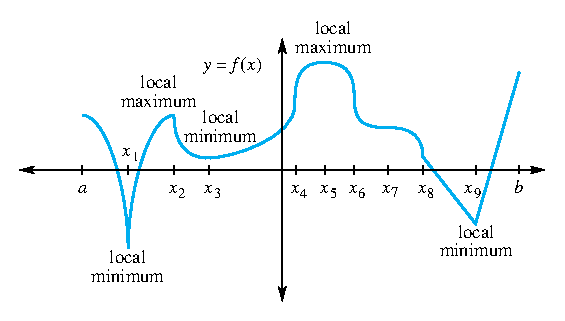
\includegraphics[width=.4\textwidth]{figsamp.eps}}
\caption{LKB1 phosphorylates Thr-172 of AMPK$\alpha$ \textit{in vitro}
and activates its kinase activity.}\label{afoto}
\end{figure}

\begin{figure*}[ht]
\begin{center}
\centerline{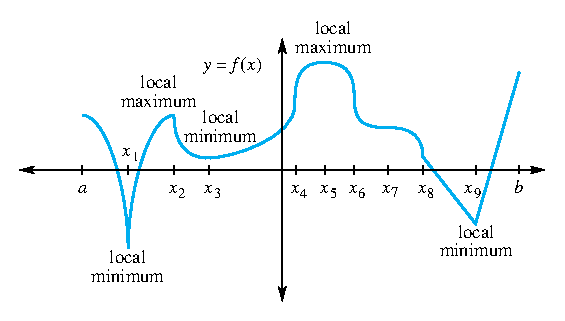
\includegraphics[width=.7\textwidth]{figsamp.eps}}
\caption{LKB1 phosphorylates Thr-172 of AMPK$\alpha$ \textit{in vitro}
and activates its kinase activity.}\label{afoto2}
\end{center}
\end{figure*}

\begin{table}[h]
\caption{Repeat length of longer allele by age of onset class.
This is what happens when the text continues.}
\begin{tabular}{@{\vrule height 10.5pt depth4pt  width0pt}lrcccc}
&\multicolumn5c{Repeat length}\\
\noalign{\vskip-11pt}
Age of onset,\\
\cline{2-6}
\vrule depth 6pt width 0pt years&\multicolumn1c{\it n}&Mean&SD&Range&Median\\
\hline
Juvenile, 2$-$20&40&60.15& 9.32&43$-$86&60\\
Typical, 21$-$50&377&45.72&2.97&40$-$58&45\\
Late, $>$50&26&41.85&1.56&40$-$45&42\tablenote{The no. of wells for all samples was 384. Genotypes were
determined by mass spectrometric assay. The $m_t$ value indicates the
average number of wells positive for the over represented allele.}
\\
\hline
\end{tabular}
\end{table}


\begin{table*}[ht]
\caption{Summary of the experimental results}
\begin{tabular*}{\hsize}
{@{\extracolsep{\fill}}rrrrrrrrrrrrr}
\multicolumn{3}{l}{Parameters}&
\multicolumn{5}{c}{Averaged Results}&
\multicolumn{5}{c}{Comparisons}\cr
\hline
\multicolumn1c{$n$}&\multicolumn1c{$S^*_{MAX}$}&
\multicolumn1c{$t_1$}&\multicolumn1c{\ $r_1$}&
\multicolumn1c{\ $m_1$}&\multicolumn1c{$t_2$}&
\multicolumn1c{$r_2$}&\multicolumn1c{$m_2$}
&\multicolumn1c{$t_{lb}$}&\multicolumn1c{\ \ $t_1/t_2$}&
$r_1/r_2$&$m_1/m_2$&
$t_1/t_{lb}$\cr
\hline
10\tablenote{Stanford Synchrotron Radiation Laboratory (Stanford University,
Stanford, CA)}&1\quad &4&.0007&4&4&.0020&4&4&1.000&.333&1.000&1.000\cr
10\tablenote{$R_{\rm FREE}=R$ factor for the $\sim 5$\% of the randomly
chosen unique ref\/lections not used in the ref\/inement.}&5\quad &50&.0008&8&50&.0020&12&49&.999&.417&.698&1.020\cr
100\tablenote{Calculated for all observed data}&20\quad &2840975&.0423&95&2871117&.1083&521&---&
.990&.390&.182&---\ \ \cr
\hline
\end{tabular*}
\end{table*}


\end{document}


